\mychapter{Credential Relationship Binding Nullifier}

While our $\MIMCABC$ system enables binding different credentials from different issuers to the same identity, practical identity systems based on Anonymous Credentials require additional structure and security properties to satisfy regulatory requirements. Real-world deployments distinguish between foundational identities like a government-Id or passport, and other credentials that depend on the foundational identity such as licenses and certificates. This hierarchy allows a system to focus security requirements like KYC/AML and revocation on the foundational identity and requiring a verifier to check the foundational identity status during verification rather than holding every credential accountable. 
This natural hierarchy exists in systems such as access control lists, delegatable credentials, federated identity models and public certificate infrastructure. We refer to foundational identities and Master Credential, $(\credm)$ and the child-credentials as Context Credentials $(\credc)$. Much focus has been on enabling anonymous credential systems with this capability \cite{crites_syra_2024, rabaninejad_attribute-based_2024, maram2021candid} privately as it's not naive, many constructions work but sacrifice efficiency with pairing computation, or sacrifice privacy to establish it. 

Furthermore, identity binding doesn't prevent Sybil attacks for users creating context credentials. Because credentials and identities are private, retaining sybil resistance of credentials is challenging in Anonymous Credentials. Non-private sybil resistance is easy, issuers can keep lists of the identifiers they've issued. However, when this information is secret, users can more easily create multiple credentials. 

Technical Gap
At the cryptographic level, implementing a privacy-preserving credential hierarchy with Sybil resistance requires a mechanism to generate unique, deterministic tokens (nullifiers) for each user-context pair without revealing user identity. This leads to our core technical challenge

\begin{center} 
    \emph{How can we construct efficient verifiable random functions (VRFs) with zero-knowledge proofs of correctness without relying on expensive pairing operations, while maintaining security for nullifier generation?}
\end{center}




\subsection{Limitations of Existing Approaches}

Verifiable Random Functions (VRFs) offer a promising foundation for nullifier construction, but existing implementations have significant limitations:

\begin{itemize}
    \item \textbf{Standard VRF:} Traditional constructions expose the user's public key during verification, breaking unlinkability during context credential issuance \cite{hutchison_verifiable_2005}

    \item CanDID \cite{maram2021candid} uses master and context credentials but sacrifices privacy by maintaining public mappings between credential identifiers and prevents sybil resistance with an MPC-PRF introducing substantial overhead

    \item \textbf{Pairing-based Approaches:} Recent constructions like UTT~\cite{tomescu2022utt} and \cite{rabaninejad_attribute-based_2024} use PRF's and bilinear pairings that, while private and secure, are computationally expensive which introduces significant overhead if multiple nullifiers are required simultaneously 
\end{itemize}





















Our approach introduces a pairing-free nullifier construction optimized for anonymous credentials, providing strong privacy guarantees with practical efficiency.


\begin{center} 
    \emph{How can we extend $\MIMCABC$ to support a credential hierarchy while enforcing efficient, privacy-preserving sybil resistance}
\end{center}


We introduce a Credential Relationship Binding Nullifier (CRBN) that:

 credentials through an efficient, pairing-free nullifier construction

Enables context-specific Sybil resistance without revealing user identity

Supports efficient revocation through the hierarchy (revoking a master credential implicitly invalidates all its context credentials)

Our construction features a novel zero-knowledge proof of multiplicative inverse that enables verification of nullifier correctness without expensive pairing operations, reducing computational overhead by 33-60\% compared to pairing-based approaches."






Previous work


\noindent This pairing-free nullifier construction extends our MIMC-ABC system with efficient Sybil resistance while maintaining privacy. Beyond preventing credential reuse, the underlying zero-knowledge proof of multiplicative inverse enables a broader class of credential relationship predicates, enhancing the expressiveness of our anonymous credential system without sacrificing performance.

\section{Problem Statement and Motivation}
Anonymous Credential systems must balance user privacy with protection against Sybil attacks, where a malicious user creates multiple credentials. In our $\MIMCABC$ based Identity System, users possess a Master Credential containing a secret key $\k$ and may obtain multiple Context Credentials for different services or contexts. Each Context Credential contains a unique identifier $\ctx$ (e.g., $\mathcal{H}(\text{``DriverLicense''})$). During issuance, the system must ensure that each user receives at most one credential per context—without compromising privacy by revealing user identities.

Specifically, we need a privacy-preserving mechanism we need that creates a unique deterministic token (nullifier) for each user-context pair without compromising anonymity.


\begin{table}
\begin{center}
\caption{Comparison of our construction over previous work.}
\label{tab:comparison-chap4}
\begin{tabular}{l|ccccc}
Features    									& 
Sybil Resist.  & 
Hierarchy & 
Private & 
Efficient Token & 
Predicate Proofs \\
\hline
CanDID \cite{maram2021candid}     				&
\ding{51}     & 
\ding{51} 	& 
\ding{55}  &  
\ding{55}     & 
\ding{55}		\\
SyRA \cite{crites_syra_2024}     				& 
\ding{51}    	& 
\ding{51}     & 
\ding{51}  &  
\ding{51}     & 
\ding{55}		\\
S3ID \cite{rabaninejad_attribute-based_2024}  & 
\ding{51}     & 
\ding{51}    	& 
\ding{55}  &  
\ding{55}     & 
\ding{55}		\\
UTT               & 
\ding{51}     & 
\ding{51}    	& 
\ding{51}  &  
\ding{55}     & 
\ding{51}		\\
Chap3             & 
\ding{55}     & 
\ding{55}    	& 
\ding{51}  &  
\ding{55}     & 
\ding{51}		\\
Ours  										& 
\ding{51}     & 
\ding{51}    	& 
\ding{51}  &  
\ding{51}     & 
\ding{51}		\\
\end{tabular}
\end{center}
\vspace{1em}
\footnotetext[1]{Predicate Proofs allow users to prove statements about their credentials privately}
\footnotetext[2]{Efficient Token refers to optimization of token verification}
\end{table}

\subsection{Contributions}

\noindent We improve the state of the art by creating a lightweight VRF construction tailored for Anonymous Credential systems with 3 contributions:
\begin{enumerate}
        \item \textbf{Pairing-Free VRF in Prime-Order Groups:} We adapt the Dodis-Yampolskiy VRF structure to function efficiently in standard prime-order groups, achieving provable pseudorandomness under the $q$-Diffie-Hellman Inversion ($q$-DHI) assumption. We show that VRF evaluation is 33\% faster and verification is 60\% faster than previous constructions.

        \item \textbf{Novel $\Sigma$-protocol for Multiplicative Inverse:} We show our problem reduces to proving a committed value equals the multiplicative inverse of another committed value and introduce an efficient zero-knowledge proof technique for proving the relation without using pairings. The protocol has value beyond our specific application, offering a new general technique for $\Sigma$-protocols requiring $q-DHI$ relationships.

         \item \textbf{Formal Security Guarantees:} maintains \emph{Pseudorandomness} of the VRF outputs in the indistinguishable outputs, \emph{uniqueness} in one nullifier per $(\k, \ctx)$ pair preventing sybil attacks

\end{enumerate}

By incorporating this innovation into our credential system, we create a Credential Relationship Binding Nullifier (CRBN) that:

\begin{enumerate}
    \item Cryptographically binds master credentials (containing key $\k$) to context credentials (with context identifiers $\ctx$) via a verifiable nullifier

    \item Enforces sybil resistance for context credentials while retaining privacy

    \item Integrates with the efficient $\Sigma$-protocols used throughout the system
    
\end{enumerate}

This extends our MIMC-ABC system into a complete identity framework with Sybil resistance and practical efficiency. 














\subsection{Construction}
During verification, the user proves in zero-knowledge that they possess a valid master credential with VRF key $\k$, a context credential with a specific $\ctx$ value and the nullifier $\nul$ is correctly formed by using a secret $\k$ in $\credm$ and $\ctx$ in $\credc$. 

\begin{equation}
\nul = g^{1/(\k + \ctx)} \in \G
\end{equation}

\subsection{Integration with Identity System}


\begin{figure}
        \begin{pchstack}[boxed, center, space=4em]
            \begin{pcvstack}
                \procedure[space=auto]{Passport}{%
                \id: 12345, \\
                \ctx: "master", \\
                \exp: "10/11/2026" \\
                \k: 54321
                }
            \end{pcvstack}
            \pcvspace
            \begin{pcvstack}
                \procedure[space=auto]{Driver License}{%
                 \id: 12345, \\
                 \ctx: "DMV", \\
                 \exp: "10/11/2028"
                }
            \end{pcvstack}
            \begin{pcvstack}
                \procedure[space=auto]{Nullifier}{%
                 \textsf{n} = 1/(\k + "DMV") \\
                 \nul = g^{\textsf{n}}
                }
            \end{pcvstack}
        \end{pchstack}
    \caption{Example Credential and Nullifier for context DMV}
    \label{fig:two-creds}
\end{figure}


\[
    \mathcal{R}_{\mathsf{vrf}} = \zkpok \left\{ 
    \begin{array}{l} 
    (\cmm, \cmc, \mathsf{N}), (\id, \ctx, , \exp, \k, r_1, r_2) \\
    \end{array} 
    \middle|
    \begin{array}{l}
        \cmm = g_1^{\id}g_2^{\ctx}g_3^{\exp}g_4^{\k}g^{r_1}  \wedge \ctx="master" \\
        \cmc = g_1^{\id}g_2^{\ctx}g_3^{\exp}g^{r_2} \wedge \ctx="DMV" \\
        \nul = g^{1/(k + \ctx)}
    \end{array} 
    \right\}
\]
    

This requires only standard group operations and leverages the proof machinery already present in our credential system, avoiding the computational cost of pairings.











\subsection{Security Properties}
Our nullifier construction provides:

\begin{itemize}
    \item \textbf{Uniqueness}: For fixed $\k$ and $\ctx$, the nullifier is deterministic and unique
    \item \textbf{Unlinkability}: Nullifiers for different contexts are unlinkable without knowledge of $\k$
    \item \textbf{Double-spending prevention}: The system can detect if the same user attempts to obtain multiple credentials for the same context
\end{itemize}

These properties follow directly from the security of our underlying commitment scheme and the algebraic properties of the multiplicative inverse. The formal security analysis extends our existing credential system model.



\subsection{Zero-Knowledge Proof of Multiplicative Inverse}
The core technical challenge in our construction is proving knowledge of $\k$ and $\ctx$ (from different commitments) such that $\nul = g^{1/(\k + \ctx)}$ without revealing these values, we do this by introducing an auxiliary variable $\n = 1/(\k + \ctx) \in \Z_p$ and proving that $\n \cdot (\k + \ctx) = 1 \quad \wedge \quad \nul = g^z$

Our $\Sigma$-protocol for this relation works as follows:

\begin{protocol}{Non-Pairing VRF Output Verification}{non-pairing-vrf-verify}\label{pok-non-pairing-vrf}
\textbf{Common Input:} Group generators $g_1, g_2, g_3, g_4, g_5, g \in \mathbb{G}$, and commitments $\cm_1, \cm_2, \cm_3, \cm_4, \cm_5, \cm_6 \in \mathbb{G}$\\
\textbf{Prover Input:} Witness $(\id, \k, \ctx, r_1, r_2, r_3, r_4, r_5, \textsf{n}, r_6)$ such that:
    \begin{align*}
        \cm_1 &= g_1^{\id} g_2^{\k} g^{r_1}     &    \cm_2 &= g_1^{\id} g_3^{\ctx} g^{r_2}  &   \cm_3 &= g_4^{\k + \ctx} g^{r_3}\\
        \cm_4 &= g_5^{\textsf{n}} g^{r_4}   &   \cm_5 &= \cm_3^{\textsf{n}} g^{r_5}     &   \cm_6 &= g^{r_6} \\
        \textsf{n} &= \frac{1}{\k + \ctx}   &   r_6 &= r_3 \cdot \textsf{n} + r_5    &   \frac{\cm_5}{\cm_6} &= g_4
    \end{align*}

\begin{enumerate}
    \item \textbf{Commitment:} Prover samples random blinding factors from $\Z_q$:
    \[
        a_x \quad \text{ for } \quad x \in \{\ \id, \k, \ctx, \textsf{n}, r_1, \ldots,r_6\} \in \Z_q
    \]
    \textbf{Computes}:
    \begin{align*}
        T_1 &\gets g_1^{a_{\id}} g_2^{a_k} g^{a_{r_1}}  &   T_2 &\gets g_1^{a_{\id}} g_3^{a_{\ctx}} g^{a_{r_2}}     &   T_3 &\gets g_4^{a_k + a_{\ctx}} g^{a_{r_3}} \\
        T_4 &\gets g_5^{a_{\textsf{n}}} g^{a_{r_4}}   &   T_5 &\gets \cm_3^{a_{\textsf{n}}} g^{a_{r_5}}     &   T_6 &\gets g^{a_{r_6}}
    \end{align*}
    Sends $(T_1, T_2, T_3, T_4, T_5, T_6)$ to verifier.
    
    \item \textbf{Challenge:} Verifier samples $c \sample \mathbb{Z}_q$ and sends to prover.
    
    \item \textbf{Response:} Prover computes:
    \[
    z_x = a_x + c \cdot x \quad \text{ for } \quad x \in \{\ \id, \k, \ctx, \textsf{n}, r_1, \ldots,r_6\} 
    \]
    Sends $(z_{\id}, z_k, z_{\ctx}, z_{r_1}, z_{r_2}, z_{r_3}, z_{\textsf{n}}, z_{r_4}, z_{r_5}, z_{r_6})$ to verifier.
    
    \item \textbf{Verification:} Verifier checks:
    \begin{align*}
        g_1^{z_{\id}} g_2^{z_k} g^{z_{r_1}} &\stackrel{?}{=} T_1 \cdot \cm_1^c 
        & 
        g_1^{z_{\id}} g_3^{z_{\ctx}} g^{z_{r_2}} &\stackrel{?}{=} T_2 \cdot \cm_2^c \\
        g_4^{z_k + z_{\ctx}} g^{z_{r_3}} &\stackrel{?}{=} T_3 \cdot \cm_3^c
        &
        g_5^{z_{\textsf{n}}} g^{z_{r_4}} &\stackrel{?}{=} T_4 \cdot \cm_4^c \\
        \cm_3^{z_{\textsf{n}}} g^{z_{r_5}} &\stackrel{?}{=} T_5 \cdot \cm_5^c
        &
        g^{z_{r_6}} &\stackrel{?}{=} T_6 \cdot \cm_6^c
        &
        \frac{\cm_5}{\cm_6} &\stackrel{?}{=} g_4
    \end{align*}
\end{enumerate}
\end{protocol}

\section{Proofs}

Theorem: Correctness

Theorem: Soundness

Theorem: Zero Knowledge

\section{Security}

Our nullifier construction builds on the Dodis-Yampolskiy VRF \cite{hutchison_verifiable_2005}, adapting it to work efficiently in standard prime-order groups without pairings. The security relies on the $q$-Diffie-Hellman Inversion ($q$-DHI) assumption, which states that given $(g, g^x, g^{x^2}, \ldots, g^{x^q})$, no PPT adversary can compute $g^{1/x}$ with non-negligible probability \cite{mitsunari_new_2002}.

\subsubsection{Security Properties}

Our nullifier construction satisfies three critical security properties:

\begin{itemize}
    \item \textbf{Uniqueness}: For fixed $\k$ and $\ctx$, the nullifier $\nul = g^{1/(\k + \ctx)}$ is deterministic, ensuring each user can generate exactly one nullifier per context. This prevents Sybil attacks where users attempt to obtain multiple credentials for the same context.
    
    \item \textbf{Pseudorandomness}: Without knowledge of $\k$, the nullifier $\nul$ is computationally indistinguishable from a random group element under the $q$-DHI assumption. This ensures that nullifiers cannot be predicted or linked to other user activities.
    
    \item \textbf{Zero-knowledge}: Our $\Sigma$-protocol proves nullifier correctness without revealing any information about $\k$ or $\ctx$, maintaining user privacy while enabling Sybil resistance.
\end{itemize}

The security of our construction follows directly from: (1) the hardness of the $q$-DHI problem in prime-order groups, (2) the correctness and soundness of our multiplicative inverse $\Sigma$-protocol, and (3) the security of our underlying commitment scheme, which ensures the binding of user credentials to their VRF key $\k$.



\subsection{Performance Analysis}
Benchmarks were performed on MacBook Air M2 16GB RAM using our Rust implementation with the arkworks library \cite{arkworks_contributors_arkworks_2022}. Compared to the state-of-the-art nullifier scheme from \cite{tomescu2022utt}, our scheme removes a pairing with a speedup of 33\% for VRF evaluation and 60\% for Verify.

\begin{table}[h!]
\centering
\label{tab:cred-rel-binding-nullifier-table}
\begin{tabular}{l@{\hspace{1.5em}}r@{\hspace{1.5em}}r@{\hspace{1.5em}}r}
\toprule
Operation & Pairing (ms) & Us (ms) & Our Speedup (\%)) \\
\midrule
Evaluate & 5.83 & 3.89 & 33.26 \\
Verify & 6.37 & 2.52 & 60.42 \\
\bottomrule
\end{tabular}
\caption{Credential Relationship Binding Nullifier Scheme Comparison}
\end{table}
\vspace{-1cm}
\begin{figure}[h!]
    \centering
    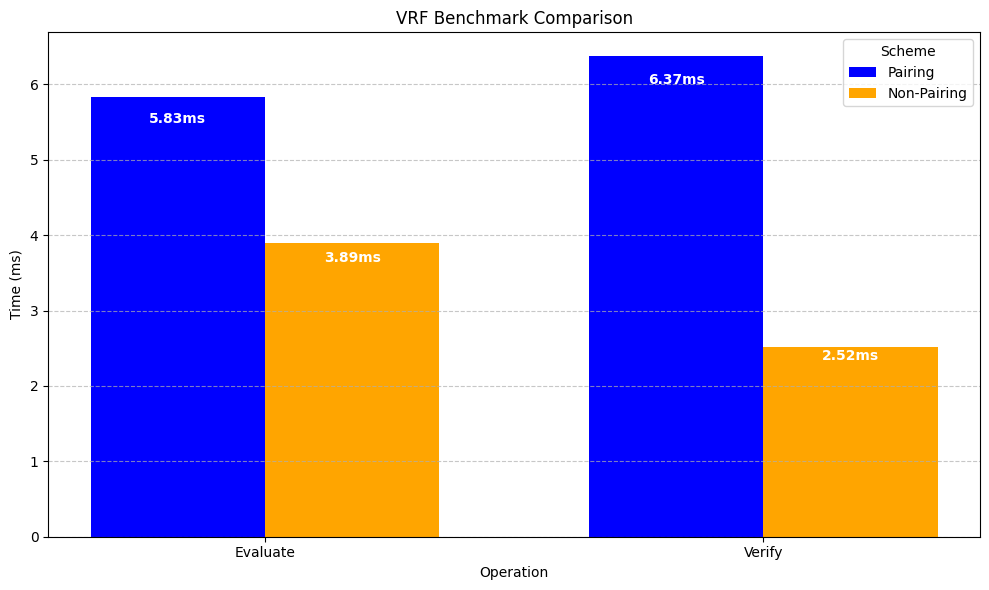
\includegraphics[width=0.75\linewidth]{figures/vrf-benchmark.png}
    \caption{VRF Benchmark}
    \label{fig:vrf-benchmark}
\end{figure}

\clearpage
